\chapter{Foundations}
\label{cha:foundations}

\todo{Add chapter introduction}

\section{Decentralized Identities}

\todo{Explain Decentralized Identities}

\section{BestRentalPoC}

The BestRentalPoC is a proof of concept for the usage of decentralized identities.
BestRental is a fictive car rental company, which requires customers to have a valid driver's license
when renting a car.
For this purpose, the driving license authority can issue a customer, called Alice, a verifiable credential (VC).
The VC is stored in Alice's digital wallet.
When renting a car, Alice can present her VC to BestRental, who can then verify the validity of Alice's driver's license.

The BestRentalPoC consists of three parts: The BestRental application, the DrivingLicenseAuthority application
and the decentralized identity system.
The BestRental application allows Alice to rent a car and present her VC.
The DrivingLicenseAuthority application allows the issuance of a VC to Alice.
Finally, the decentralized identity system provides the functionality of issuing and verifying VCs.

The BestRental application consists of a browser-based frontend and a microservice, which handles the required
business logic. In the same way, the DrivingLicenseAuthority application consists of a frontend and a microservice.
Additionally, both applications have tenants in Microsoft Azure which include an Azure Active Directory and
a Key Vault called VerifiedIDVault.

The decentralized identity system consists of Microsoft Entra Verified ID and the Trust System called DidWeb.
This proof of concept utilizes Microsoft Entra Verified ID to implement decentralized identities.
Entra provides all services which are required for this. This includes services to issues and to verify VCs.

Figure \ref{fig:sps_architecture_bestrental} shows the SystemPlusSoftware Architecture of the Demonstrator BestRental.

\begin{figure}
	\centering
	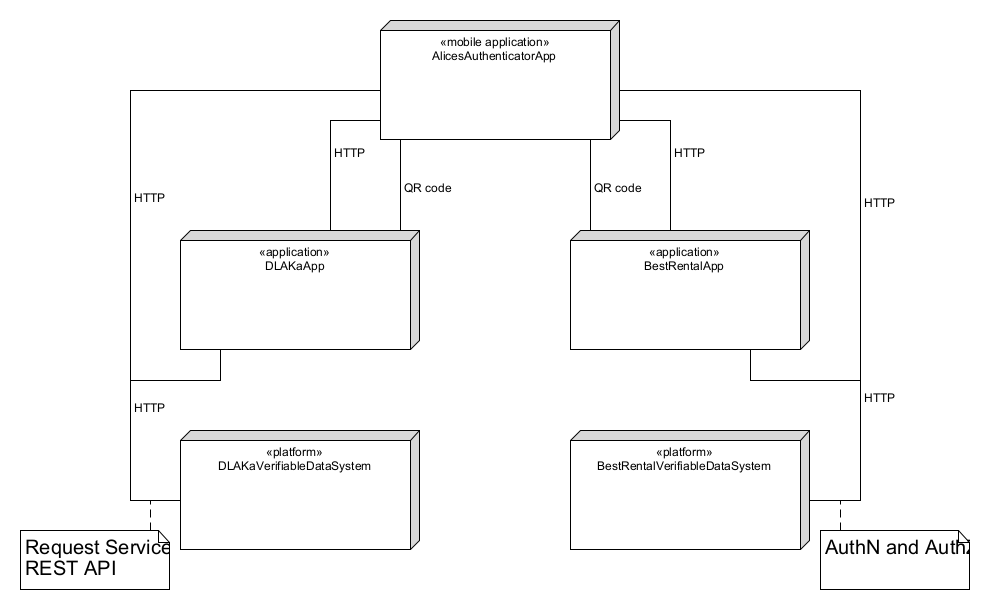
\includegraphics[width=\textwidth]{figures/sps_BestRentalPOC.png}
	\caption{SystemPlusSoftware Architecture BestRental}
	\label{fig:sps_architecture_bestrental}
\end{figure}

\section{Monitoring}

\todo{Cleanup and actually write this section}

According to \cite{9837035}, observability consists of three pillars: Metrics, Logs, and Traces.
Metrics.
Logs are streams of textual information emitted by an application. They can contain information about important
events, like an incoming request, or provide details about the occurrence of exceptions.
Traces are a way of tracking the path of requests through a system. A trace contains detailed information
about all the services that were called during the processing of a request and can be thought of
as a stack trace for microservices.

Because of the scope of this work, only Metrics will be used. Logs and Traces will still be considered
in the development of a solution so that they may be added in the future.

Because of the scope of this work, only the pillar of Metrics is considered.

\begin{quote}
\textit{``Metrics are numerical representations of data that Ops teams use to determine the overall behavior of a system, service, or network component over time.'', \cite{9837035}}
\end{quote}

The four golden signals \cite{Beyer2016-xi}
\begin{itemize}
    \item Latency: time to service a request
    \item Traffic: requests per second
    \item Errors: rate of failed requests
    \item Saturation: how saturated are constrained resources like memory or I/O
\end{itemize}

White-box vs. Black-box Monitoring \cite{Beyer2016-xi}
\begin{itemize}
    \item White-box: Monitoring based on internal system metrics.
    \item Black-box: Monitoring based on externally visible behavior.
\end{itemize}

Internal vs. External resources in a monitoring context:
Internal resources describe resources that allow direct access to their internals.
An example of an internal resource is a self-hosted microservice.
External resources describe resources that do not allow direct access to their internals.
An example of an external resource is a Software-as-a-Service (SaaS) product which is used in a context that should be monitored.

External resources can, because of their nature, only be monitored using the Black-box approach.
Internal resources however can be monitored with both the White-box and Black-box approach.

Motivations for monitoring cloud applications \cite{6483656}
\begin{itemize}
    \item Capacity and Resource Planning
    \item Capacity and Resource Management
    \item Data Center Management
    \item SLA Management
    \item Billing
    \item Troubleshooting
    \item Performance Management
    \item Security Management
\end{itemize}

\todo{Capacity and Resource Planning}

\todo{Capacity and Resource Management}

Data Center Management is mainly concerned with the efficient usage of resources.
One key measurement of the efficiency of a data center is its energy efficiency.

SLA Management refers to the monitoring of parameters, which are defined in Service Level Agreements (SLA).
These parameters must be within set bounds for an SLA to be considered fulfilled.

Billing refers to the monitoring of parameters that influence the cost of running an application.
When an application is hosted on a cloud provider's Infrastructure-as-a-Service (IaaS) system,
one of those parameters might be the number of compute instances that an application uses.

While Troubleshooting usually refers to the tracing of requests and failures to provide a dataset for analyzing and fixing issues in an application,
Monitoring can also be used to aid in troubleshooting by recording the number of failed requests and their context.

\todo{Performance Management}

\todo{Security Management}

\section{Use Cases}

\subsection{Motivation}
The DrivingLicenseAuthorityKarlsruhe (DLAKa) wants to provide citizens with digital driving licenses,
which can, for example, be used to prove to a car rental company that they possess a valid driving license.
They hire the company ServiceProvider (SP) to develop and operate the system necessary for issuing and verifying
digital driving licenses. The contract specifies an initial payment for the development of the system
and afterward a yearly fee for the operation of the system.
After receiving the contract from DLAKa, SP starts designing the system
for DLAKa. Because SP has to operate the system on a fixed yearly budget,
they want to monitor the performance of the system to identify parts with excessive resource usage, which
incur additional costs. They identify the CPU and memory usage of the system as two technical metrics that should be monitored.
Additionally, DLAKa has asked them to provide the capability of monitoring business metrics for them.
DLAKa wants to know how many digital driving licenses are being issued and how often the issuance of a digital
driving license fails. To monitor both technical and business metrics, SP designs the ServiceProviderMonitor (SPMonitor) as a part
of the system for DLAKa which will provide all functionality for monitoring the specified metrics.

BestRental, a car rental company, has heard of DLAKa's plans for digital driving licenses
and wants to integrate them into its online rental system. Contrary to DLAKa, BestRental develops its
system in-house. Similarly to DLAKa, BestRental is interested in obtaining business metrics from its system.
They want to use these metrics to make business decisions like if they should increase the capacity of their fleet in the future.
For this purpose, BestRental designs an additional application called BestMonitor that will provide all the monitoring functionality.
In the beginning, they are only interested in one metric: How many active rentals are there?

For the design of SPMonitor, SP created two use cases: Present Metric and Collect Metric.
The relation of these use cases can be seen in the Use Case Diagram in Figure \ref{fig:use_case_monitoring_dlakaapp}.
Present Metric handles the use case of presenting the collected metrics to a user, this is described in Listing \ref{lis:use_case_description_present_metric}.
Collect Metric is concerned with how SPMonitor receives metrics for later presentation to a user, this is described in Listing \ref{lis:use_case_description_collect_metric}.

The metrics that will initially be monitored by SPMonitor are the number of issued digital driving licenses (NumDDL)
and the memory usage of the DLAKaApp (MemUse). The NumDDL metric is a business metric for DLAKa, while MemUse is
a technical metric that allows SP to monitor the performance of DLAKaApp.

\begin{figure}
	\centering
	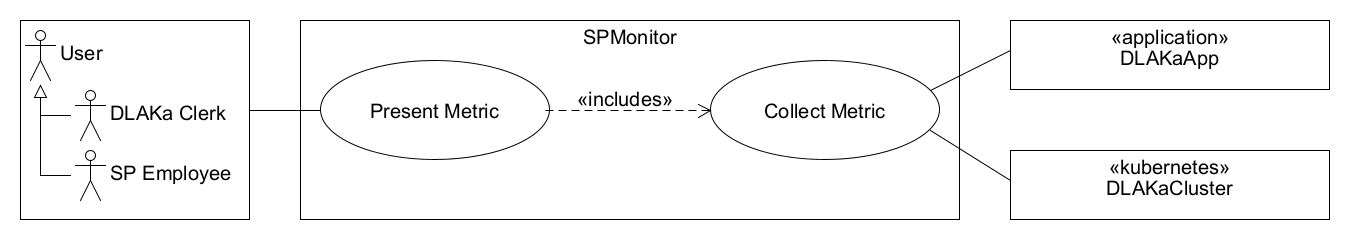
\includegraphics[width=\textwidth]{figures/2.1_use_case_spmonitor.png}
	\caption{Use Case Diagram: SPMonitor}
	\label{fig:use_case_monitoring_dlakaapp}
\end{figure}

\subsection{Use Case Present Metric}
\todo{Elaborate}

\begin{lstlisting}[caption = {Use Case Description: Present Metric}, label = {lis:use_case_description_present_metric}, style = kit-cm, language=] 
Title: Present Metric

Primary Actors: DLAKa Clerk

Preconditions:
- SPMonitor has the NumDDL metric configured

Flow:
1. DLAKa Clerk opens the dashboard for the NumDDL metric
2. SPMonitor retrieves all stored values for the NumDDL metric
3. SPMonitor displays the values in a graph

Alternative Flows:
2a. SPMonitor has no values stored for the NumDDL metric
2a1. SPMonitor displays a message that the NumDDL metric has no stored values

Information Requirements:
- Values for the NumDDL metric
\end{lstlisting}

\subsection{Use Case Collect Metric}
\todo{Elaborate}

\begin{lstlisting}[caption = {Use Case Description: Collect Metric}, label = {lis:use_case_description_collect_metric}, style = kit-cm, language=] 
Title: Collect Metric

Secondary Actors: DLAKaApp, DLAKaCluster

Preconditions:
- DLAKaApp is set up to collect the NumDDL metric
- DLAKaCluster is set up to collect the MemUse metric
- DLAKaApp is running inside of the DLAKaCluster
Postconditions:
- SPMonitor has values stored for NumDDL and MemUse

Flow:
1. SPMonitor sends a request to DLAKaApp for the NumDDL metric
2. DLAKaApp replies with a value for the NumDDL metric
3. SPMonitor receives the reply
4. SPMonitor stores the value for the NumDDL metric
5. SPMonitor sends a request to DLAKaCluster for the MemUse metric
6. DLAKaCluster replies with a value for the MemUse metric
7. SPMonitor receives the reply
8. SPMonitor stores the value for the MemUse metric

Alternative Flows:
2a. DLAKaApp replies with an error message
2a1. SPMonitor receives the error message
2a2. SPMonitor retries to request the NumDDL metric
6a. DLAKaCluster replies with an error message
6a1. SPMonitor receives the error message
6a2. SPMonitor retries to request the MemUse metric

Information Requirements:
- Value for the NumDDL metric
- Value for the MemUse metric
\end{lstlisting}

\section{DevOps}